% ! TeX root = document.tex
\documentclass[aspectratio=169, 9pt]{beamer}
% ! TeX root = ...
\usepackage[utf8]{inputenc}
\usepackage{multicol}
\usepackage{roboto}
\usepackage{fontawesome5}
\usepackage{tikz}
\usepackage[backend=bibtex,sorting=none,style=numeric,doi=true]{biblatex} 
\usepackage{adjustbox}
\usepackage{minted}
% ! TeX root = ../document.tex
\title{Towards Pulverised Architectures for Collective Adaptive Systems through Multi-tier Programming}
\author[G.Aguzzi]{
  \textbf{Gianluca Aguzzi}\inst{1} \and
  Roberto Casadei\inst{1} \and
  Danilo Pianini\inst{1} \\
  Guido Salvaneschi\inst{2} \and
  Mirko Viroli\inst{1}
}
\institute{
  \inst{1}
  \texttt{Alma Mater Studiorum} -- Università di Bologna, Cesena, Italy \\
  \inst{2}
  University of St.Gallen: St.Gallen, Switzerland
}
\date{October 1, 2021}
% ! TeX root = ../document.tex
\usetheme{material}
\useLightTheme
\usePrimaryBlueGrey
\useAccentIndigo
\addbibresource{biblio.bib}
\begin{document}
% ! TeX root = ../document.tex
\begin{frameImg}{img/background.jpg}
  \titlepage
\end{frameImg}

\section{Overview}
% ! TeX root = document.tex
\begin{frameImg}{img/background.jpg}
  \begin{card}[Collective Adaptive Systems]
    {
      \color{accent} ``Refer to a form of complex systems where 
      a \textit{large number} of \textit{heterogeneous} entities interact without specific \textit{external} or \textit{internal} 
      central control, adapt their behaviour to environmental 
      settings in pursuit of an \textit{individual} or \textit{collective} goal."}\footnote{\url{http://unige.ch/cui/cas/}
    } 
  \end{card}
\end{frameImg}

\section{Challenges}
% ! TeX root = ../document.tex
\begin{frame}<6>{Challenges}
  %% Background
  \only<1-4>{ 
    \begin{backgroundblock} 
      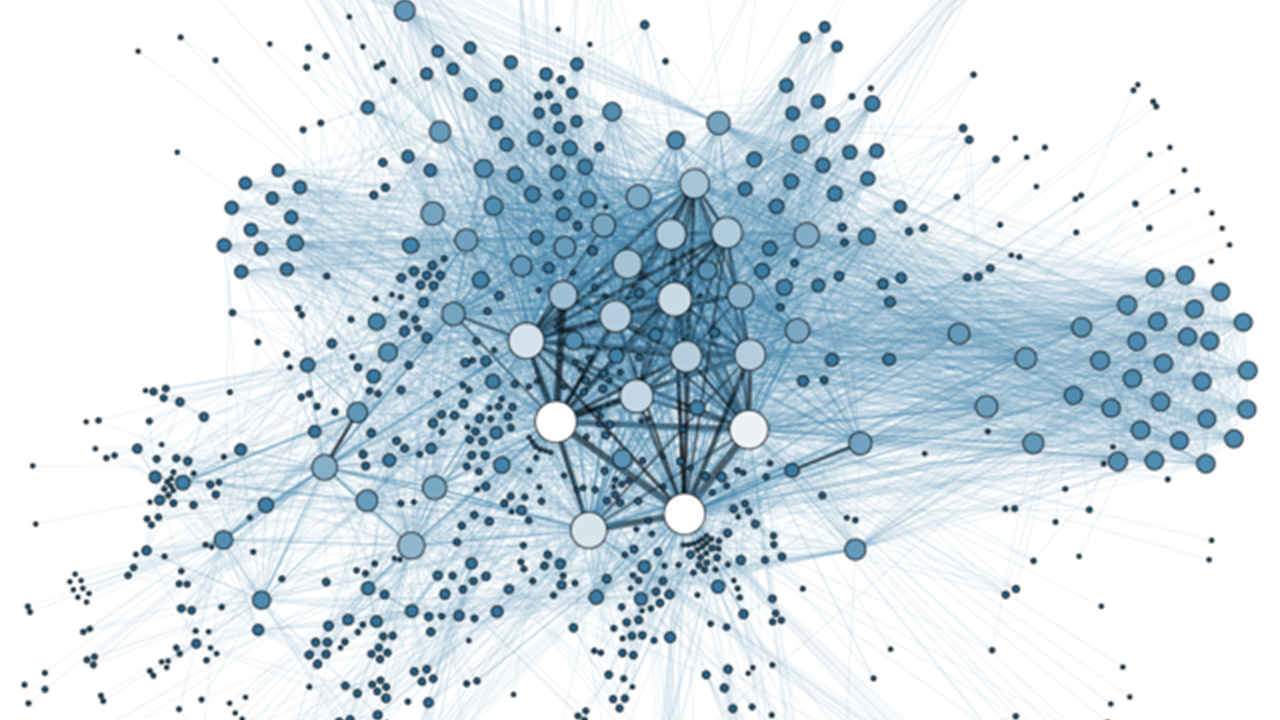
\includegraphics[width=\paperwidth]{img/complex-network.png} 
    \end{backgroundblock} 
  }
  \only<5-6>{ 
    \begin{backgroundblock} 
      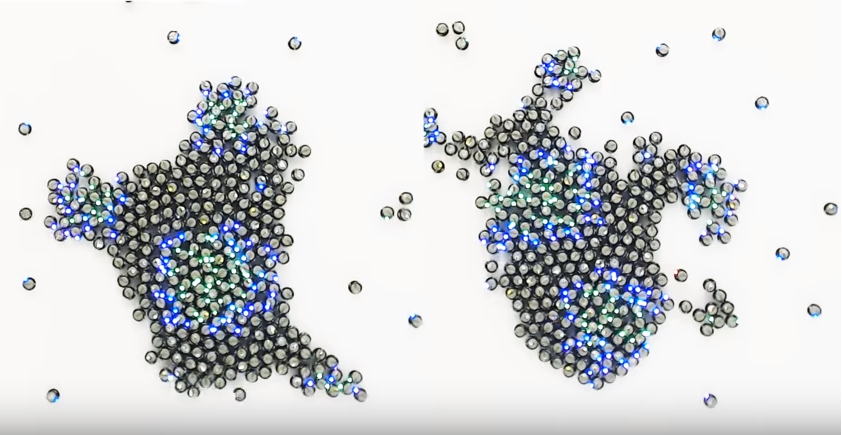
\includegraphics[height=\paperheight]{img/swarms.png}
    \end{backgroundblock} 
  }
  \begin{card}
    \begin{itemize}
      \item<1-> Complex and layered networks
      \begin{itemize}
        \item <2->Large scale
        \item <3->Heterogenous
        \item <4->Dynamic
      \end{itemize}
      \item<5-> Distributed control
      \item<6-> Environmental changes
    \end{itemize}
  \end{card}
\end{frame}

\section{Proposed approach}
% ! TeX root = ../document.tex
\begin{frame}{Proposed approach}
  %% Main content
  \begin{cardTiny}
    \begin{itemize}
      \item<1-> Describe the collective behaviour with {\color{accent} \textit{Aggregate Computing}~\cite{DBLP:journals/jlap/ViroliBDACP19}}
      \item<2-> Define your concrete deployment with {\color{accent} \textit{Multi-tier programming}~\cite{DBLP:journals/csur/WeisenburgerWS20}}
      \item<3-> Inject the {\color{accent} \textit{same}} collective behaviour in different deployments thanks to {\color{accent} \textit{Pulverisation}~\cite{DBLP:journals/fi/CasadeiPPVW20}}
    \end{itemize}
  \end{cardTiny}
  %% Images
  \begin{columns}[onlytextwidth, t]
    \begin{column}{0.27\textwidth}
      \begin{adjustbox}{max width=\textwidth, valign=m, margin=0}
        \cardImg{img/aggregate-computing-file}{\textwidth}
      \end{adjustbox}
    \end{column}
    \begin{column}{0.32\textwidth}
      \begin{adjustbox}{max width=\textwidth, valign=m}
        \presentationGraphics{img/scalaloci}{1}{1}
      \end{adjustbox}
    \end{column}
    \begin{column}{0.25\textwidth}
      \begin{adjustbox}{max width=\textwidth, valign=m}
        \presentationGraphics{img/finalidea}{1-2}{1}
      \end{adjustbox}
    \end{column}
  \end{columns}
\end{frame}

\section{Aggregate Computing}
% ! TeX root = ../document.tex
\begin{frame}{Proposed approach}
  %% Main content
  \begin{cardTiny}
    \begin{itemize}
      \item<1-> Describe the collective behaviour with {\color{accent} \textit{Aggregate Computing}~\cite{DBLP:journals/jlap/ViroliBDACP19}}
      \item<2-> Define your concrete deployment with {\color{accent} \textit{Multi-tier programming}~\cite{DBLP:journals/csur/WeisenburgerWS20}}
      \item<3-> Inject the {\color{accent} \textit{same}} collective behaviour in different deployments thanks to {\color{accent} \textit{Pulverisation}~\cite{DBLP:journals/fi/CasadeiPPVW20}}
    \end{itemize}
  \end{cardTiny}
  %% Images
  \begin{columns}[onlytextwidth, t]
    \begin{column}{0.27\textwidth}
      \begin{adjustbox}{max width=\textwidth, valign=m, margin=0}
        \cardImg{img/aggregate-computing-file}{\textwidth}
      \end{adjustbox}
    \end{column}
    \begin{column}{0.32\textwidth}
      \begin{adjustbox}{max width=\textwidth, valign=m}
        \presentationGraphics{img/scalaloci}{1}{1}
      \end{adjustbox}
    \end{column}
    \begin{column}{0.25\textwidth}
      \begin{adjustbox}{max width=\textwidth, valign=m}
        \presentationGraphics{img/finalidea}{1-2}{1}
      \end{adjustbox}
    \end{column}
  \end{columns}
\end{frame}

\section{Pulverisation}
% ! TeX root = document.tex
\begin{frame}{Pulverisation~\cite{DBLP:journals/fi/CasadeiPPVW20}}
  \begin{cardTiny}
    {
      \color{accent} An approach proposed for Aggregate Computing 
      to neatly separate behavioural and deployment concerns. 
    }
  \end{cardTiny}
  \begin{columns}
    \begin{column}{0.45\textwidth}
      \presentationGraphics{img/logical-system.jpg}{1}{1}
    \end{column}
    \begin{column}{0.38\textwidth}
      \presentationGraphics{img/deployments}{1-2}{1}
    \end{column}
  \end{columns}
  \only<3>{} 
\end{frame}

\section{Multi-tier programming}
% ! TeX root = ../document.tex
\begin{frame}{Multi-tier programming~\cite{DBLP:journals/csur/WeisenburgerWS20}}
  \begin{cardTiny}
  \highlight {
    A programming approach by which distributed architectures 
    are defined in a single compilation unit with a single language. 
  }
  \end{cardTiny}
  \centering
  \cardImg{img/multitier}{0.35\textwidth}
\end{frame}

\section{Framework choosen}
% ! TeX root = /document.tex
\begin{frame}{Frameworks}
  \begin{card}[ScaFi~\cite{DBLP:conf/isola/CasadeiVAD20} (Scala Field)]
    A tool-chain comprised by a Domain Specific Language that supports field-calculus.
  \end{card}
  \pause
  \begin{card}[ScalaLoci~\cite{Weisenburger.2018}]
    A langauge extension to enable compile-time multi-tier programming.\\
    %The  structure of  a ScalaLoci application is defined through \textit{peers} and \textit{ties}
  \end{card}
\end{frame}

\section{Puliverised architectures}
% ! TeX root = ...
\begin{frame}[fragile]{Puliverised architectures: \textbf{logical components}}
  \begin{columns}
    \begin{column}{0.7\textwidth}
      \begin{cardTiny}
        \begin{minted}[fontsize=\footnotesize]{scala}
@multitier trait LogicalSystem {
  @peer type LNode <: { type Tie <: Multiple[LNode] }
}
@multitier trait PulverisedSystem 
 extends LogicalSystem {  
  @peer type SensorComponent        <: LNode 
  @peer type ActuatorComponent      <: LNode
  @peer type StateComponent         <: LNode
  @peer type BehaviourComponent     <: LNode
  @peer type CommunicationComponent <: LNode
}
        \end{minted}
      \end{cardTiny}
    \end{column}
    \begin{column}{0.3\textwidth}
      \cardImg{example-image-a}{\textwidth}
    \end{column}
  \end{columns}
\end{frame}
% ! TeX root = /document.tex
\begin{frame}[fragile]{Puliverised architectures: \textbf{concrete deployments}}
  \begin{columns}

    \begin{column}{0.3\textwidth}
      \cardImg{example-image-b}{\textwidth}
    \end{column}
    \begin{column}{0.7\textwidth}
      \begin{cardTiny}
        \begin{minted}[fontsize=\footnotesize]{scala}
@multitier object IoTSystem extends PulverisedSystem {
  @peer type Thin <: { type Tie <: Multiple[Thick] }
  @peer type Thick <: { 
    type Tie <: Multiple[Thick] with Multiple[Thin]
  }
  // Pulverised component allocation on devices
  @peer type SensorComponent <: Thin
  @peer type ActuatorComponent <: Thin
  @peer type StateComponent <: Thick
  @peer type BehaviourComponent <: Thick
  @peer type CommunicationComponent <: Thick
}
        \end{minted}
      \end{cardTiny}
    \end{column}
  \end{columns}
\end{frame}
% ! TeX root = ../document.tex
\begin{frame}[fragile]{Puliverised architectures: \textbf{concrete deployments}}
  \begin{columns}
    \begin{column}{0.58\textwidth}
      \begin{cardTiny}
        \begin{minted}[fontsize=\footnotesize]{scala}
@multitier object BrokerBased extends PulverisedSystem {
  @peer type Node <: { type Tie <: Single[Broker] }
  @peer type Broker <: { 
    type Tie <: Multiple[Node] with Multiple[Broker] 
  }
  // Pulverised component allocation on devices
  @peer type SensorComponent <: Node
  @peer type ActuatorComponent <: Node
  @peer type StateComponent <: Node
  @peer type BehaviourComponent <: Node
  @peer type CommunicationComponent <: Broker
}
        \end{minted}
      \end{cardTiny}
    \end{column}
    \begin{column}{0.43\textwidth}
      \cardImg{img/example-2}{\textwidth}
    \end{column}
  \end{columns}
\end{frame}

\section{Conclusion}
% ! TeX root = document.tex
\begin{frame}{Conclusion}
  \begin{card}[Benefits]
    \begin{itemize}
      \item<1-> Collective behaviours are defined regardless of the IT architecture
      \item<2-> Deployments specification is declarative and type-safe thanks to Scala Loci
    \end{itemize}
  \end{card}
  \pause
  \begin{card}[Future Works]
    \begin{itemize}
      \item <3-> Opportunistic deployment and reconfiguration of the pulverised system
      \item <4-> Bring this example from a prototype to a usable library
    %  \item <5-> Continue the direction of separate the functional and non-functional aspect of application
    \end{itemize}
  \end{card}
\end{frame}


% ! TeX root = /document.tex
\begin{frame}[allowframebreaks]
  \frametitle{References}
  \printbibliography
\end{frame}
  
\end{document}